
% %%%%%%%%%%%%%%%%%%%%%%%%%%%%%%%%%%%%%%%%%%%%%%%%%%%%%%%%%%%%%%%%%%%%%%%%%
% %           Capítulo 2: MARCO TEÓRICO - REVISIÓN DE LITERATURA
% %%%%%%%%%%%%%%%%%%%%%%%%%%%%%%%%%%%%%%%%%%%%%%%%%%%%%%%%%%%%%%%%%%%%%%%%%

\chapter{Fundamentos Previos}

En este capítulo se da la teoría preliminar necesaria que forma las bases del problema a atacar. Se comienza en la Sección \ref{sec:Dominancia_Pareto} describiendo de manera formal un problema de optimización multiobjetivo, en la siguiente Sección \ref{sec:clasif_MOO} se explica una clasificación breve de algoritmos usados para optimizar problemas multiobjetivo visto desde la perspectiva de la estrategia usada para resolverlo; es decir, cuándo se usan las preferencias del tomador de decisiones para buscar las soluciones. Después, en la Sección \ref{sec:Escalarizaciones}, se explican escalarizaciones comunes, haciendo énfasis en la función aumentada de Tchebycheff que se usará frecuentemente en este trabajo. 
Se concluye el capítulo en la Sección \ref{sec:AE} con una explicación breve de qué son los algoritmos Evolutivos.



\section{Optimización multiobjetivo} \label{sec:MOO}



La \textbf{optimización} es una rama de las matemáticas aplicadas y de la computación, dedicada a encontrar métodos efectivos para realizar tareas específicas. Esto incluye, por ejemplo, optimizar algoritmos o minimizar errores a través de la adecuada configuración de parámetros.

Tradicionalmente, la optimización se ha centrado en \textit{problemas de objetivo único} (SOP por sus siglas en inglés), por su simplicidad y la factibilidad de encontrar soluciones. Sin embargo, la realidad muestra que la mayoría de los problemas son de un carácter \textit{multiobjetivo} (MOP por sus siglas en inglés), dada su complejidad y múltiples metas involucradas.

Atender un problema únicamente desde una perspectiva SOP puede resultar en una simplificación excesiva. El enfoque de MOP permite capturar la complejidad real del problema, ofreciendo una visión más integral y representativa del entorno en el que se desenvuelve.

Definiremos formalmente los componentes de un MOP en la Sección \ref{sec:Dominancia_Pareto}, explorando cómo este enfoque puede proporcionar soluciones más completas y realistas a problemas complejos. Después, en la Sección \ref{sec:clasif_MOO} explicaremos una clasificación de algoritmos multiobjetivo en términos generales. Luego, definiremos escalarizaciones comúnes que también usaremos para definir el algoritmo usado en este trabajo en la Sección \ref{sec:Escalarizaciones}.

Concluiremos el capítulo en la Sección \ref{sec:AE}, explicando los algoritmos evolutivos que usaremos en este trabajo para encontrar encontrar una solución a un MOP (los algoritmos son llamados MOEAs por sus siglas en inglés). 

Para tratar este problema desde una aplicación específica a ciencia de datos tomaremos el siguiente ejemplo de selección de características en un problema de clasificación:

\begin{texample} \label{ex:Selecc}
    Dado un conjunto de datos con $n$ columnas y un algoritmo de k-medias con dos componentes, etiqueta en una de dos clases (0 o 1). El problema de selección de características consiste en encontrar el menor número de columnas posibles tal que el error de clasificación sea mínimo.
    
    Así, tenemos que minimizar dos objetivos: el número de características y el error de clasificación, volviendo a esto un problema de optimización biobjetivo. 
\end{texample}


\subsection{Elementos de un problema multiobjetivo: definición matemática} \label{sec:Dominancia_Pareto}

Un problema de optimización multiobjetivo busca encontrar, dadas unas funciones y restricciones, el conjunto de puntos que minimicen dichas funciones bajo estas restricciones. Puede ser caracterizado de manera más formal por las siguientes definiciones, que son ilustradas en la Figura \ref{fig:dec_obj}  \footnote{Imagen tomada de \cite{coelloEvolutionaryAlgorithmsSolving}}. 

\begin{itemize}
    \item \textbf{Región de decisión o factible}, $Q\subseteq \mathbb{R}^n$; corresponde a la región que cumple restricciones $g,f$ que se explican en la siguiente viñeta. 
    
    $$ Q=\left\{x\in \mathbb{R}^n|g_i(x)\leq 0, h_j(x)=0 , 0\leq i \leq n, 0\leq j \leq n,\right\}.$$ 

    La región factible es donde cambian las variables de entrada para intentar optimizar los objetivos. Las funciones que aparecen como condiciones extra se explican en la siguiente viñeta.\\ En el Ejemplo \ref{ex:Selecc} de selección de características  el espacio factible sería una máscara binaria sobre las columnas que usamos (con un 1) y las que no (con un 0). De modo que el espacio está dado por todos los $x\in Q$ tales que  $Q=\{0,1\}^n$.
    \item \textbf{Restricciones} sobre el dominio que se pueden escribir como $J$ restricciones de \textbf{igualdad} e $I$ de \textbf{desigualdad} mediante la siguiente ecuación  
    \begin{align*}
        g_i(x)\leq 0, \ \ i\in\{1,\ldots,I\},\\  h_j(x)=0 ,\ \ j\in{1,\ldots,J}.
    \end{align*} 
    \item Las $m$ \textbf{funciones objetivo} que buscaremos minimizar a través del siguiente mapeo$$ F=(f_0,\ldots,f_{m-1}):Q\rightarrow \mathbb{R}^m. $$
    \item \textbf{Espacio de objetivos}, la imagen de la región factible a través de las funciones objetivo 
     $$F(Q)=\{F(x) | x \in Q\}.$$
     
    Es donde se puede interpretar o evaluar el desempeño del algoritmo. En el Ejemplo \ref{ex:Selecc} tenemos dos objetivos, el primer objetivo $f_0$ que mide el tamaño del conjunto, es decir, las características usadas. El segundo objetivo $f_1$ es el error de clasificación del modelo de modo que conjuntamente viven en $(f_0(x),f_1(x))\in \mathbb{R}^2$.
    
\end{itemize}

\begin{figure}[H]
    \centering
    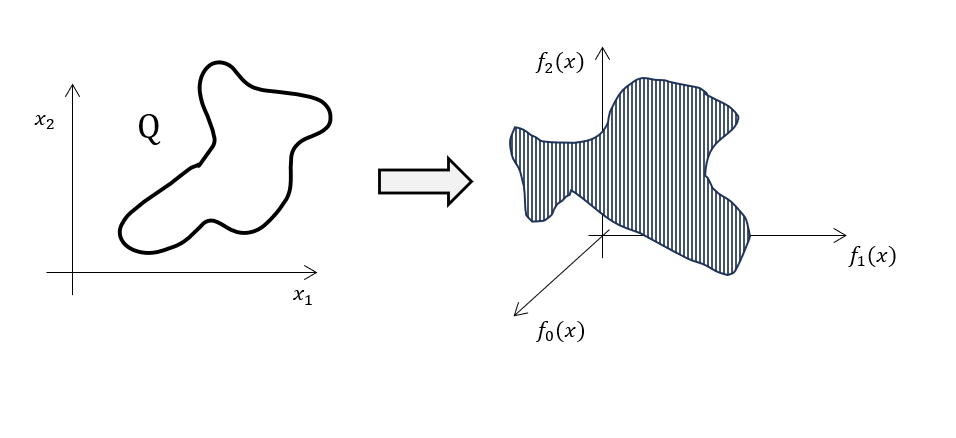
\includegraphics[width=\textwidth]{Figuras/obj_dec.png}
    \caption[Ilustración de un MOP]{Ilustración de un MOP con el espacio factible y el de objetivos. }
    \label{fig:dec_obj}
\end{figure}

Con estos elementos, la finalidad de resolver un problema de optimización multiobjetivo es encontrar el conjunto de vectores en la región factible tal que minimice cada uno de ellos, es decir

\begin{equation} \label{eq:MOO}
    \min_{x\in Q} \{F(x)\}.
\end{equation}

En nuestro Ejemplo \ref{ex:Selecc} buscamos encontrar el vector binario de características tal que minimice tanto el número de columnas usadas por el modelo, así como el error de clasificación. 

Esta definición puede ser fácilmente adaptada al caso donde intentamos maximizar algunos objetivos en vez de minimizarlos. Podemos convertir una objetivo de maximización en uno de minimización haciendo una reflexión en esa dirección; es decir, si el objetivo $i$ se maximizara, podemos obtener un problema de minimización al hacer la siguiente transformación $f_i \rightarrow -f_i$. 

La Ecuación \eqref{eq:MOO} no tiene porque tener solución única. Para convencernos de esto, basta ver la Figura \ref{fig:pareto} y pensar en el caso en el que tenemos dos vectores $x_1, x_2$ tales que $P_1=(f_0(x_1),f_1(x_1)), P_2=(f_0(x_2),f_1(x_2))$. En este caso como podemos ver en la Figura \ref{fig:pareto} $f_0(x_1)< f_0(x_2)$, pero $f_1(x_1) > f_1(x_2)$; es decir, $x_1$ es menor en el primer objetivo que $x_2$, sin embargo, $x_2$ tiene menor segundo objetivo que $x_1$. Así, se vuelve evidente que la meta de la optimización multiobjetivo no será encontrar un punto sino un conjunto de puntos tales que ninguno sea mejor que otro en ambos objetivos.

\begin{figure}[H]
    \centering
    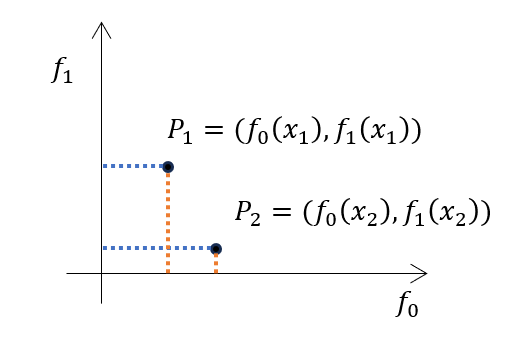
\includegraphics[scale=.5]{Figuras/pareto.png}
    \caption[Vectores en el espacio de objetivos]{Vectores en el espacio de objetivos. .}
    \label{fig:pareto}
\end{figure}


Misma que se puede formular con diferentes niveles cada vez más estrictos de qué significa que un punto domine a otro. Las listamos a continuación:

Para comprender el objetivo de los algoritmos multiobjetivo, es útil recurrir a una analogía social propuesta por Pareto en 1927\footnote{Esta perspectiva se enfoca en el punto de vista \emph{a posteriori}, que se explorará más adelante en la Sección \ref{sec:clasif_MOO}. En otras palabras, tras identificar soluciones para un problema, seleccionamos aquellas que mejor se ajusten a nuestros objetivos.}. Imaginemos una población de $N$ individuos y nuestro desafío es garantizar un estado donde cada uno alcance el máximo bienestar posible. En una sociedad compleja, cualquier cambio en el bienestar de una persona inevitablemente afecta a los demás. Por ejemplo, aumentar la riqueza de un individuo frecuentemente implica redistribuir recursos de otros. Bajo este contexto, Pareto define el estado ideal como aquel donde ninguna persona puede incrementar su bienestar sin perjudicar a otra. Esto se traduce matemáticamente en la noción de \textbf{optimalidad de Pareto}. A continuación mostraremos diferentes definiciones de optimalidad de Pareto en formas cada vez más estrictas, es decir, cada vez se le pide más a un punto para que se considere "mejor" que otro. 


\subsubsection*{Dominancia de Pareto}

\begin{itemize}
    \item Un vector $x\in Q$ es \textbf{preferido} a otro vector $y\in Q$, denotado por $x<_p y \, \, $ si $\, x_i <y_i, \forall i$. De manera análoga se define uno que es menor o igual, denotado por $x\leq_p y$.
    \item Un vector $x\in Q$ \textbf{domina fuertemente} a otro vector $y\in Q$, denotado como $x < y$ con respecto a un MOP como \eqref{eq:MOO}, si sus objetivos son preferidos, es decir, si $F(x) <_p F(y)$.
    \item Un vector $x\in Q$ \textbf{domina} a otro $y\in Q$, denotado $x\prec y$, con respecto a un MOP si $F(x) \leq_p F(y)$ y $F(x)\neq F(y)$, en otro caso se dice que $y\in Q$  es \textbf{no-dominado} por $x\in Q$.
    \item Un vector $x\in Q$ \textbf{domina débilmente} a $y\in Q$, denotado $x\preceq y$ si $F(x)\leq_p F(y)$. Es decir, permitimos el caso donde los puntos sean iguales. 
\end{itemize}

Esto nos da varias nociones de un vector siendo mejor que otro, mientras mejor sea nuestro algoritmo, mayor tenderá hacia la primera definición ya que es más estricta que el resto como podemos ver en la siguiente ecuación

\begin{equation} \label{eq:contencion_def_pareto}
    x <_p  y \implies x \prec y \implies x \preceq y. \nonumber
\end{equation}

\begin{definition}
Diremos que una solución $x\in Q$ es \textbf{óptima de Pareto} si es tal que se cumple
\begin{equation} \label{eq:opt_pareto}
    \nexists \,\, y\in Q \,\, \text{ tal que } y\prec x. \nonumber
\end{equation}

Es decir, no existe ninguna forma de mejorar sin empeorar.
\end{definition}

\begin{definition}
Al conjunto de todos los puntos del espacio factible que son óptimos de Pareto se le conoce como \textbf{Conjunto de Pareto} y a su imagen a través de un MOP, definido en la Ecuación \ref{eq:MOO}, se le conoce como \textbf{Frente de Pareto}. Formalmente se definen como:

El conjunto de Pareto es el conjunto de todas las soluciones óptimas de Pareto, es decir
\begin{equation} \label{eq:pareto_set}
    P=\{x\in Q \, \, \big| \, \, x \text{ Es una solución óptima de Pareto del MOP}\}, \nonumber
\end{equation}

mientras que la imagen del conjunto de Pareto a través de las funciones objetivo es el frente de Pareto 

\begin{equation} \label{eq:pareto_front}
F(P)=\{y\in \mathbb{R}^m \, \, \big| \, \, y=F(x), x \text{ es una solución óptima de Pareto del MOP}\}.    \nonumber
\end{equation}

\end{definition}

El frente de Pareto de un MOP está acotado por dos puntos de referencia: el vector ideal y el vector de Nadir que definimos a continuación y pueden ser visualizados en la Figura \ref{fig:vectores_referencia} (Definiciones y Figura ambas tomadas de \cite{tesis_phd_guillermo}).


\begin{definition} \label{def:Ideal}
    El \textbf{Vector Ideal} vive en el espacio de objetivos y se denota por $z^*\in \mathbb{R}^m$ se define como 
    
    $$z^*_i=\min_{x\in Q}\, f_i(x), \,\, i=1,2,\ldots,m .$$
\end{definition}

\begin{definition} \label{def:Nadir}
    El \textbf{Vector de Nadir} vive en el espacio de objetivos y se denota por $z^{\text{nad}}\in \mathbb{R}^m$ se define como 
    
    $$z^*_i=\max_{x\in \text{PS}}\, f_i(x), \,\, i=1,2,\ldots,m ,$$

    donde $\text{PS}$ es el conjunto de Pareto.
\end{definition}

Estos dos puntos representan la combinación del mejor y el peor de los casos por cada objetivo. Es decir, no es necesario que existan como parte del mapeo del espacio factible. Además a veces es conveniente definir  otro punto que domina al ideal (y por consecuencia al de Nadir) y lo definimos a continuación

\begin{definition} \label{def:utopico}
    Dado el punto ideal $z^*$ y un vector positivo $$\epsilon=(\epsilon_1,\ldots,\epsilon_m) , \epsilon_i>0 \,\, \forall i \in \{1,\ldots,m\},$$
    el \textbf{Vector Utópico} se define como 

    $$ z^{**}=z^*-\epsilon .$$
\end{definition}

\begin{figure}[H]
    \centering
    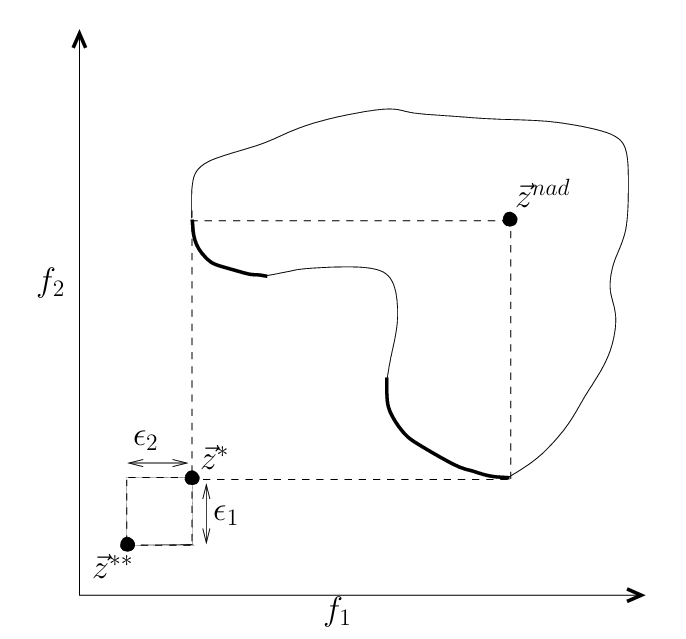
\includegraphics[scale=0.5]{Figuras/nadir_ideal_utopico.png}
    \caption{Vectores de referencia: vector ideal $z^*$, vector de nadir $z^{\text{nadir}}$, vector utópico $z^{**}$.}
    \label{fig:vectores_referencia}
\end{figure}

En general, bajo ciertos supuestos, el frente de Pareto suele formar un espacio de \emph{una} dimensión menor al número de objetivos, aunque esto no es necesario.

\subsection{Clasificación de algoritmos multiobjetivo} \label{sec:clasif_MOO}

Al aproximarse a la solución de un problema multiobjetivo, salen naturalmente maneras de dividir las estrategias de solución que son últiles para abordar el problema. Por ejemplo, podemos dividir los algoritmos por el \textbf{número de soluciones} \cite{talbiMetaheuristicsDesignImplementation2009} que generan paso a paso:

\begin{itemize}
    \item \textbf{Una solución}: Estos métodos generan sólo una solución en cada paso, como los métodos de gradiente descendiente en SOP.
    \item \textbf{Basados en poblaciones}: Se va generando un conjunto de aproximación al frente de Pareto en cada uno de los pasos del algoritmo. Dentro de estos algoritmos se encuentran los evolutivos de los que hablaremos en la Sección \ref{sec:AE} del siguiente capítulo. 
\end{itemize}

Como la salida de un MOP no suele ser una solución puntual, es útil pensar el problema desde la perspectiva de una persona (o más en general un sistema) que, dado un conjunto de aproximación, seleccionará algún subconjunto de este espacio para resolver su problema dadas sus preferencias. Es decir, haciendo alusión al Ejemplo \ref{ex:Selecc}, teniendo el frente de Pareto podría ser conveniente tomar un subconjunto con mayor número de características, pero menor error, si estas fueran nuestras preferencias.  A la persona encargada de evaluar los diferentes intercambios que surgen de evaluar los diferentes objetivos de acuerdo a sus preferencias se le denomina el \textbf{tomador de decisiones} (DM por sus siglas en inglés). 

También podemos categorizar los MOP a través de cómo servimos al tomador de decisiones. Así, obtenemos las siguientes categorías

\begin{itemize}
    \item \textbf{A priori}: Las preferencias del tomador de decisiones se toman en cuenta antes de iniciar la búsqueda del frente de Pareto. Esto puede ser útil ya que podemos integrar su preferencia directamente en el algoritmo y así usar optimización mono-objetivo para guiar la búsqueda.
    \item \textbf{A posteriori}: Dado el resultado del algoritmo multiobjetivo (la aproximación al frente de Pareto), se selecciona el resultado que va mas de acuerdo a las preferencias del DM.
    \item \textbf{Interactivo}: Tanto el optimizador como el DM trabajan en conjunto. Primero se buscan algunas soluciones, que son evaluadas por el DM para guiar la búsqueda. 
\end{itemize}


\subsection{Escalarizaciones} \label{sec:Escalarizaciones}

Una de las maneras más sencilla de resolver un problema multiobjetivo es trasladarlo a uno con un solo objetivo y ahí usar todos los resultados existentes en el área de optimización mono-objetivo. A esto se le conoce como escalarización ya que trasladamos el problema vectorial de $\mathbb{R}^m$ a uno escalar en $\mathbb{R}$. El resultado de un SOP suele ser sólo un punto, sin embargo, nosotros estamos buscando un método que nos devuelva una aproximación al frente de Pareto. Para ayudarnos con esta tarea podemos definir varias escalarizaciones de forma que se vaya obteniendo una representación diferente del frente en cada SOP único.

Se puede, por ejemplo, hacer una \textbf{suma ponderada} \cite{zadehOptimalityNonscalarvaluedPerformance1963} de los objetivos, para tener
\begin{align} \label{eq:suma_ponderada}
    min f_\alpha(x):=\sum_{i=1}^m \alpha_i f_i(x), x\in Q,
\end{align}
donde los $0\leq \alpha_i$ son coeficientes positivos que determinan la proporción de la preferencia que tiene el DM por cada uno de los objetivos, de modo que suman a 1 $\sum a_i=1$ . 

Una escalarización que resultará útil en lo que sigue recibe el nombre de \textbf{método ponderado de Tchebycheff} \cite{bowmanRelationshipTchebycheffNorm1976}. Su objetivo es buscar un punto cuya imagen esté tan cerca posible a un vector de referencia. Como veremos recurrentemente en este trabajo, los algoritmos que usan un punto de referencia tienen una dependencia muy grande de qué tan buenos seamos determinando dicho punto. Está dado por
\begin{equation} \label{eq:tch_meth}
    \min_{x\in Q} \max_{i=1,\ldots,m} \alpha_i |f_i(x)-z_i|, \nonumber
\end{equation}
donde los $\alpha_i$ satisfacen las mismas restricciones de la suma ponderada y $z$ corresponde al punto de referencia. Una elección de punto de referencia  que permite a este método acceder al frente de Pareto es aquel punto que consiste en los valores mínimos en cada objetivo, es decir el vector ideal de la Definición \ref{def:Ideal}:

\begin{equation} \label{eq:vector_utopico}
    F^*=(f_1^*,\ldots,f_k^*)=(\min_x f_1(x), \ldots \min_x f_k(x)). \nonumber
\end{equation}

Podemos extender esta definición a través de la función aumentada de Tchebycheff dada por
\begin{equation} \label{eq:tchebychev}
    \text{ATCH}_{\vec{w}}=\max_{i=0,\ldots,d} \{w_ix_i\}+\alpha \sum_{i=1}^k x_i   ,
\end{equation}
donde podemos entender el segundo término como una penalización del valor de los objetivos parecido a la regularización L1 que se realiza en modelos de regresión.


% metodo de conjuntos, directed search, metodos de continuación



\section{Algoritmos Evolutivos} \label{sec:AE}

Esta sección y la siguiente siguen la parte introductoria de \cite{EAforMOEAs}. El diseño de un algoritmo evolutivo proviene del hecho de observar  que la naturaleza ha podido tener un éxito enorme produciendo complejidades increíblemente variadas y adaptables con su mecanismo de evolución natural. De este modo, un programa que vaya cambiando de acuerdo a las reglas de la evolución natural, podría tener mucho éxito. Un algoritmo evolutivo tiene las componentes necesarias para hacer esta analogía concreta y su objetivo es ir cambiando una población de individuos de manera que se encuentren los más aptos. Así, tenemos las siguientes definiciones, ilustradas en la Figura \ref{fig:EA_components} \footnote{Imagen obtenida  de \cite{coelloEvolutionaryAlgorithmsSolving}}

\begin{itemize}
    \item \textbf{Individuo}: es una solución de algún problema que se encuentra codificada. Representaciones comunes incluyen la binaria y la real. En el Ejemplo \ref{ex:Selecc} de selección de características  la representación es binaria.
    \item \textbf{Genotipo}: La representación del individuo codificada. Análogo al perfil genético de un organismo natural. 
    \item \textbf{Fenotipo}: La representación del individuo cuando es decodificado. Análogo a las características expresables de un organismo en la naturaleza. En el Ejemplo \ref{ex:Selecc} el fenotipo sería la representación en el espacio de los objetivos $f_1, f_2$.
    \item \textbf{Cromosomas}: Está formado de uno o más genotipos.
    \item \textbf{Genes}: Lo que forma a los cromosomas, cuyo valor recibe el nombre de \textbf{alelo} y puede tomar valores de un alfabeto genético dado. Análogo a cómo los alelos biológicos tienen cuatro nucleótidos: Guanina, Adenosina, Citosina y Tiamina. 
\end{itemize}

\begin{figure}[H]
    \centering
    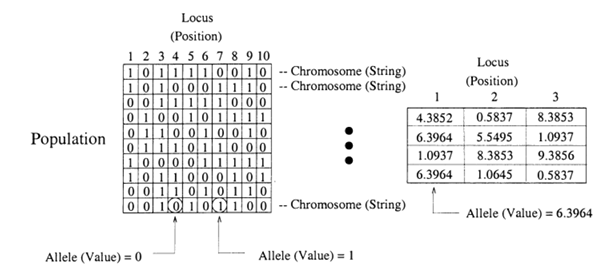
\includegraphics[width=\textwidth]{Figuras/EA_components.png}
    \caption[Componentes algoritmo evolutivo]{Descripción de componentes de la representación interna de un algoritmo evolutivo. En la parte izquierda tenemos una representación binaria, mientras que en la derecha una representación real de los individuos.}
    \label{fig:EA_components}
\end{figure}

Los algoritmos evolutivos cuentan con tres mecanismos para imitar la evolución natural que se representan en forma de diagrama en la Figura \ref{fig:EA_mech}, esta Figura fue traducida y adaptada de \cite{coelloEvolutionaryAlgorithmsSolving}. A continuación detallamos estos mecanismos: 

\begin{enumerate}
    \item Selección: Toma una función de aptitud $f$ que indica que tan bueno es cada individuo y se queda con los mejores con diferentes mecanismos como torneos. Al seleccionar los mejores individuos estamos reforzando algún camino escogido, invitando a que las futuras generaciones miren cerca de esa región del espacio de estados donde se encontró algo valioso. Este concepto, de buscar más donde ha habido mejores resultados es conocido como \textbf{Explotación}. En la Figura \ref{fig:explotacion} vemos 3 puntos en azul a los que se les permite dar 20 pasos de descenso de gradiente. Como vemos, de estos tres puntos se obtiene 
    un mínimo local. En este caso hubiera sido mejor buscar en el espacio de estados más, en vez de usar nuestras primeras opciones \\El mecanismo de selección tiene imita el proceso evolutivo biológico de la \emph{supervivencia del más apto}.
    \item Mutación: Se modifica de manera aleatoria el genotipo del individuo. Este procedimiento podría desviarnos de un individuo con una función de aptitud alta, sin embargo, la aleatoriedad hace que podamos buscar en más partes del espacio de búsqueda y no nos quedemos en un mínimo local. A esta estrategia de expandir el espacio de búsqueda se le conoce como \textbf{Exploración}. En la Figura \ref{fig:explotacion} vemos un análogo al de la Figura de \ref{fig:explotacion} sólo que en esta caso se ponen 10 puntos a explorar. De estos 10 puntos uno se encuentra cerca del último valle y puede obtener el máximo global. El balance de los dos es lo que un buen algoritmo evolutivo tendría idealmente. \\ El mecanismo de mutación es análogo a la mutación biológica, cuando se producen errores en la copia del código genético y estas modificaciones muestrean el espacio de posibilidades para un ser vivo.   
    \item Cruza: Se seleccionan dos individuos y se mezclan sus genes. Aquí también hay varios métodos, como cruza en $n$ puntos, etc. La cruza tiene un componente de explotación y de exploración ya que la combinación de dos genotipos no necesariamente dará como resultado a la misma combinación de sus fenotipos, podemos encontrar cosas inesperadas y en ese sentido tendría un aspecto de exploración. La parte que si mantiene de los individuos exitosos tendría un componente más de explotación. \\La cruza tiene un análogo natural en la reproducción de los seres vivos, la combinación de sus genes. 
\end{enumerate}

\begin{figure}[H]
    \centering
    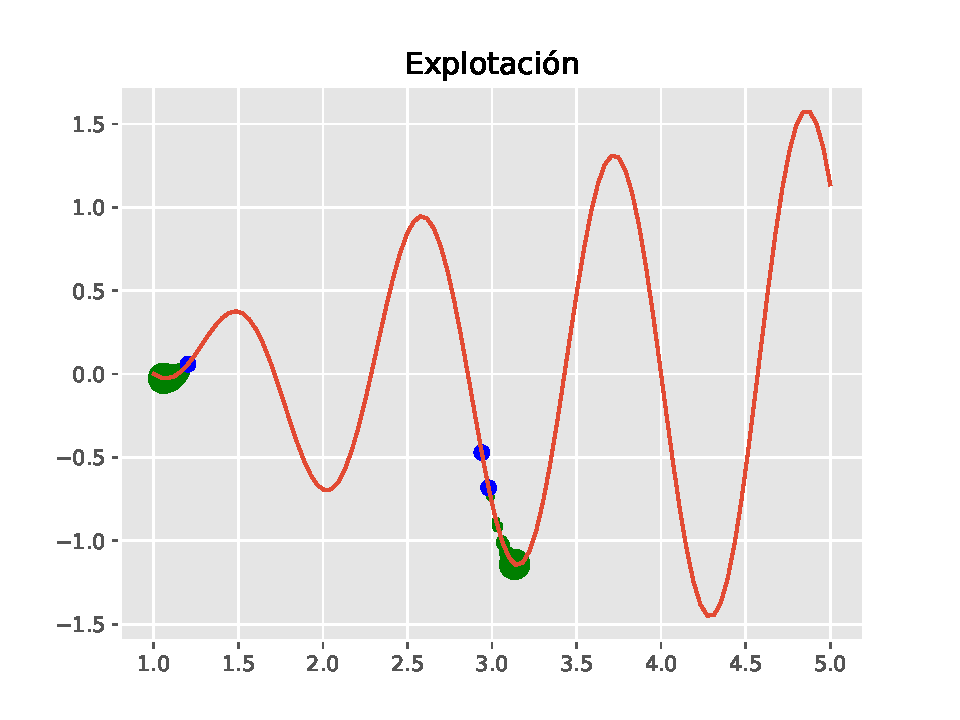
\includegraphics[width=\textwidth]{Figuras/explotacion.pdf}
    \caption[Explotación]{Estrategia de Explotación visualizada; dados los puntos haz más pasos de gradiente descendiente con ellos.}
    \label{fig:explotacion}
\end{figure}

\begin{figure}[H]
    \centering
    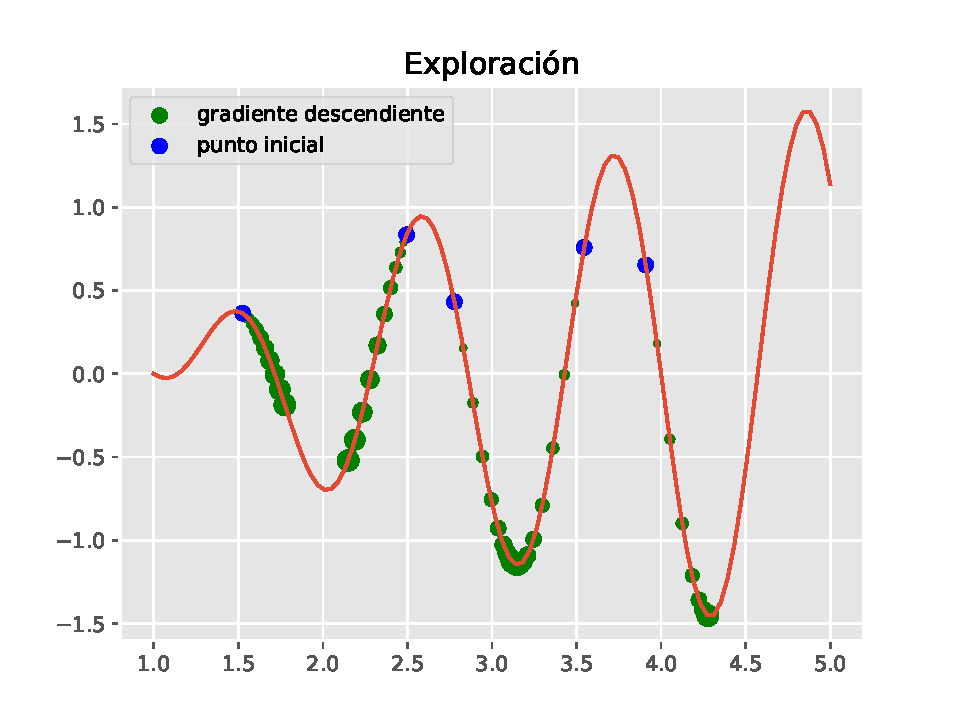
\includegraphics[width=\textwidth]{Figuras/exploracion.pdf}
    \caption[Exploración]{Estrategia de Exploración visualizada; dar menos pasos, pero desde más puntos.}
    \label{fig:exploracion}
\end{figure}

\begin{figure}[H]
    \centering
    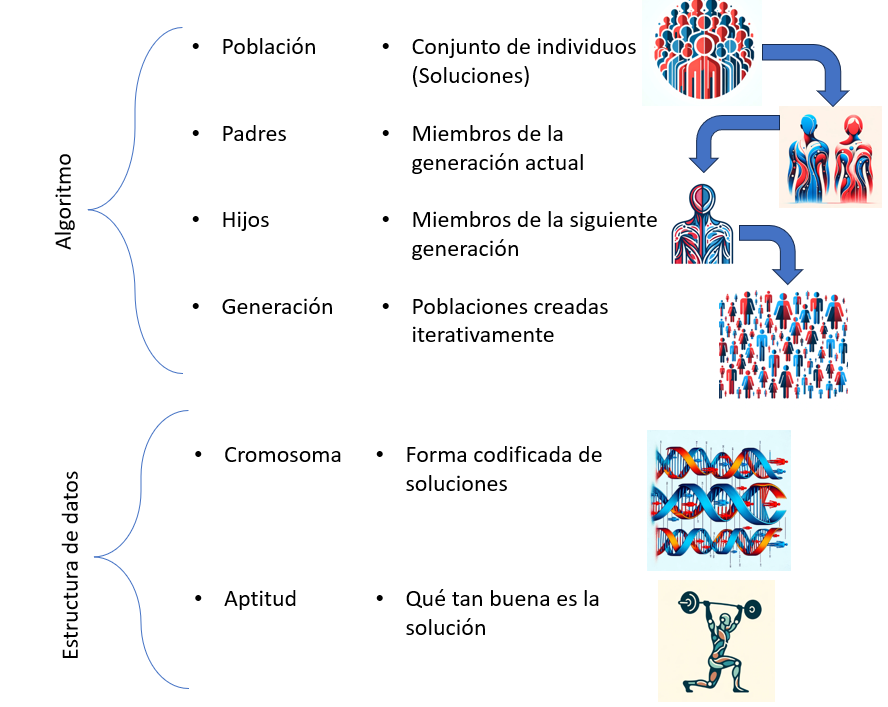
\includegraphics[width=\textwidth]{Figuras/AE_parts_algorithm.png}
    \caption{Ilustración del mecanismo básico del algoritmo evolutivo. }
    \label{fig:EA_mech}
\end{figure}

De manera formal definimos un algoritmo evolutivo de la siguiente forma \cite{coelloEvolutionaryAlgorithmsSolving}:


\begin{itemize}
    \item Sea $I$ un conjunto no vacío; el espacio de individuos. Un miembro de este conjunto, es decir, un inficiduo, vivirá en un espacio vectorial de dimensión igual a la del genotipo donde cada entrada corresponde a un gen dentro de un cromosoma. Así un individuo se denota como $\vec{a}$ y una población de $n$ individuos como como $\{\vec{a}_1,\ldots , \vec{a}_n\}$.
    \item Al ser un proceso iterativo indexamos las diferentes generaciones de individuos con el símbolo $i\in\mathbb{N}$.
    \item También denotamos como $I^\mu$ al conjunto de $\mu$ individuos. Así ${(I^{\mu})}^{(i)}$ corresponde a los $\mu$ individuos de la $i$-ésima generación. 
    \item $\{\mu^{(i)}\}, i\in \mathbb{N}$ una sucesión en $\mathbb{Z}^+$; el tamaño de las poblaciones de los padres. 
    \item $\phi: I\rightarrow R$; la función de aptitud.
    \item $\Psi: \bigcup_{i=1}^\infty (I^{\mu})^{(i)}\rightarrow \{0,1\}$; el criterio de término, 0 si no ha terminada y 1 si ya terminó. Es decir, la función $\Psi$ asigna a cada configuración de individuos una bandera de si el algoritmo debe continuar o no. Cuando se obtiene el desempeño deseado, la bandera cambiaría a verdadero (o el valor 1) y el algoritmo se detiene. 
    \item $m^{(i)}$; una sucesión de operadores de mutación, con sus respectivos parámetros. Este operador aumenta la \textbf{exploración} ya que nos permite muestrear otra parte del espacio de estados sin tomar en cuenta la aptitud de la función actual.
    \item $s^{(i)}$; una sucesión de operadores de selección, con sus respectivos parámetros. Este operador  se enfoca en la \textbf{explotación} porque toma en cuenta las soluciones que ya tienen buen desempeño en el espacio de estados para continuar el algoritmo. 
    \item $r^{(i)}$; una sucesión de operadores de recombinación, con sus respectivos parámetros. Es decir, el operador que toma dos poblaciones y mezcla los individuos para producir una nueva población.  En este caso se tiene una combinación de exploración y explotación. Por un lado, se explora porque se produce un individuo nuevo con cierto grado de aleatoriedad (dependiendo del mecanismo explícito de recombinación esto puede ser mayor o menor). Por otro lado, fomenta la explotación al combinar elementos que ya pasaron una prueba se delección. 
    \item $\chi$ un booleano que indica si el algoritmo tomará sólo la población actual o también la anterior para seleccionar los más aptos.
\end{itemize}

Entonces el pseudocódigo del algoritmo evolutivo general está dado por

\begin{algorithm}
    \caption{Algoritmo Evolutivo}\label{alg:EA}
    \begin{algorithmic}[1] % The number indicates line numbering step
    \State t:=0;
    \State Inicializa $P(0):=\{a_1(0),\ldots,a_\mu(0)\} \in I^{\mu^{(0)}}$;
    \While{$\Psi(\{P(0),\ldots,P(t)\}) \neq 1 $} \do ; 
        \State $\textit{recombina}: P'(t)=r^{(t)}(P(t))$;
        \State $\textit{muta}: P''(t)=m^{(t)}(P'(t))$;
        \State $\textit{selecciona}$:
            \If{$\chi$}
                \State $P(t +1):= s^{(t)}(P''(t))$;
                \Else  $P(t +1):= s^{(t)}(P''(t) \cup P(t))$
            \EndIf
    $t=t+1$;    
    \EndWhile
    \textbf{EndWhile}
\end{algorithmic}
\end{algorithm}

El Algoritmo \ref{alg:EA} sigue los pasos descritos a continuación: El proceso inicia con la inicialización del contador de generaciones en $t=0$. Seguidamente, se establece la primera población de individuos, donde cada uno se identifica con un subíndice que denota su posición en una población de tamaño $\mu$ y se anota entre paréntesis el número de la generación correspondiente, que para esta fase inicial es la generación 0. En la tercera línea del algoritmo, se establece que, mientras la condición de paro $\Psi$ devuelva 0, el proceso de generación de nuevos individuos continúa. Las líneas 4 y 5 están dedicadas a aplicar los operadores de recombinación y mutación, respectivamente. Del paso 6 al 9, se ejecuta el operador de selección, donde la función de aptitud $\phi$ está implícita como parte de este proceso. Este proceso depende de la bandera $\chi$: si $\chi$ es verdadera, la selección se realiza únicamente a partir de la nueva población; en cambio, si $\chi$ no es verdadera, la selección incluye tanto a los nuevos individuos como a aquellos de la generación anterior. Finalmente, se incrementa el contador de selección y el algoritmo se mantiene en este estado operativo hasta que la condición de paro deja de cumplirse y se sale del bucle \textit{While}.

Una distinción importante que hay que realizar para algoritmos evolutivos es cuando en cada paso de selección de población, se retienen los mejores individuos de la generación actual o si se sustituyen completamente con sus descendientes. Al primer tipo de algoritmos se les conoce como \textbf{elitistas} y los otros son conocidos como \textbf{no-elitistas}. Se les suele distinguir por la siguiente notación $(\mu+\lambda)$ significa que los hijos competirán por $\mu$ lugares (es decir es elitista) mientras que la notación $(\mu,\lambda)$ significa que se sustituirán los $\mu$ padres con $\lambda$ hijos. La idea detrás de los algoritmos elitistas es no perder información valiosa que se haya obtenido a lo largo del proceso de búsqueda, en este sentido podría ser considerado como una parte más de explotación sin llegar a enfocarse mucho en una parte del espacio de búsqueda. Sólo manteniendo la referencia de que en esa parte del espacio había una avenida que vale la pena explorar con operadores de mutación y cruza que fomentan la exploración.
    
Los algoritmos evolutivos se han usado para resolver problemas multiobjetivo por su enfoque en poblaciones y aproximaciones en casos donde no se puede encontrar una solución analítica. El primer algoritmo evolutivo multiobjetivo (MOEA por sus siglas en inglés) fue dado por David Schaeffer en 1984 en su tesis doctoral \cite{schafferMultipleObjectiveOptimization1984}, su propuesta llamada VEGA (Vector Evaluation Genetic Algorithm) y pretendía resolver problemas de aprendizaje de máquina.

En el Ejemplo \ref{ex:Selecc} que se ha estado revisando de hacer una selección de características de un problema de clasificación  ha sido abordado usando algoritmos evolutivos desde 1985 \cite{SIEDLECKI1989335} aunque en este caso se pretendía como un problema SOP con una restricción en el número de columnas. 


Para definir un MOEA basta cambiar la definición de la función de selección $\phi$ en el algoritmo evolutivo usual presentada en el Algoritmo \ref{alg:EA}. Esta función es la de aptitud, que ahora en el caso multiobjetivo, tendrá que ser evaluada en muchos objetivos. Así tenemos que pasamos de $\phi:I\rightarrow \mathbb{R}$ a

$$\phi:I\rightarrow \mathbb{R}^{n_{obj}}, \quad n_{obj}>1.$$


Podemos ver una descripción pictórica en la Figura \ref{fig:MOEA_EA}.

\begin{figure}[H]
    \centering
    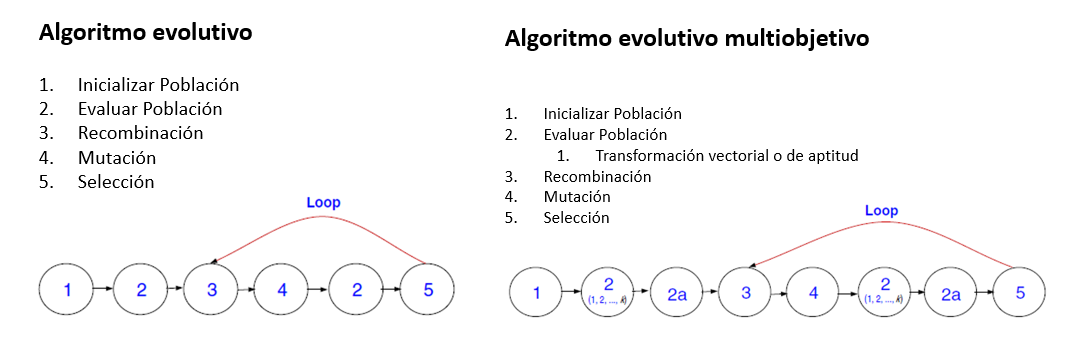
\includegraphics[width=\textwidth]{Figuras/MOEA_EA.png}
    \caption[MOEAs vs EAs]{Diferencia entre los procedimientos para uno a) y múltiples objetivos b). La diferencia es la transformación y evaluación vectorial. Imagen traducida de \cite{coelloEvolutionaryAlgorithmsSolving}.}
    \label{fig:MOEA_EA}
\end{figure}


En el contexto de algoritmos evolutivos para problemas multiobjetivo se le suele llamar \textbf{conjunto de aproximación} a la población que se obtiene paso a paso. Denotamos $\Psi$ al conjunto de todas las aproximaciones; es decir, al conjunto de todos los conjuntos finitos del espacio objetivo. Además se le llama \textbf{aproximación al frente de Pareto} a aquel $\psi$ en el conjunto de aproximación $\Psi$ tal que no existe ninguna solución en $\psi$ que domine a otra. 




